\chapter{Implementation Strategy}

The implementation strategy is based on one principle: keep the prototype readable enough that every major gameplay responsibility can be traced to a small number of Unity scripts. This section therefore focuses on code structure and the concrete trade-offs that shaped the current prototype.

\section{Code Structure}

At repository level, the project is intentionally split so that the Unity implementation, report sources, and evidence records do not collapse into one mixed file tree. The simplified WR2-relevant top-level layout used during report closeout is:

\begin{Verbatim}[fontsize=\small]
Unity-Project
|-- coursework
|-- artifacts/uml
`-- doc/src
    |-- project-records
    |-- wr1-latex
    `-- wr2-latex
\end{Verbatim}

This repository layout keeps the playable Unity project inside \texttt{coursework}, stores diagrams and report evidence separately, and makes it easier to package the repository for different audiences later. Within that structure, the current gameplay scripts are organised into a small set of folders under \texttt{coursework/Assets/Scripts}. The directory tree below reflects the current runtime structure used by the prototype.

\begin{Verbatim}[fontsize=\small]
Assets/Scripts
|-- Cards
|   |-- CardData.cs
|   |-- CardResolver.cs
|   `-- DeckManager.cs
|-- Common
|   `-- GameEnums.cs
|-- Core
|   |-- GameRoot.cs
|   `-- TurnManager.cs
|-- Grid
|   |-- GridManager.cs
|   `-- TileView.cs
|-- UI
|   |-- BattleUI.cs
|   `-- CardButtonView.cs
`-- Units
    |-- EnemyAI.cs
    `-- UnitController.cs
\end{Verbatim}

This structure intentionally mirrors responsibilities rather than future-proof architecture. The \texttt{Core} folder owns scene bootstrapping and turn flow. \texttt{Grid} owns tile generation, occupancy, and range queries. \texttt{Cards} owns card data, deck state, and explicit card resolution. \texttt{Units} owns health, team, and enemy decision logic. \texttt{UI} acts as the glue between player input and runtime state.

A file-tree view is used here deliberately. This prototype is built around a small set of scene-bound Unity \texttt{MonoBehaviour} scripts, so the clearest way to communicate structure is to show where gameplay responsibilities live under \texttt{Assets/Scripts}. A more traditional inheritance-heavy class diagram would suggest an architectural depth that the current prototype does not actually have.

\begin{figure}[H]
\centering
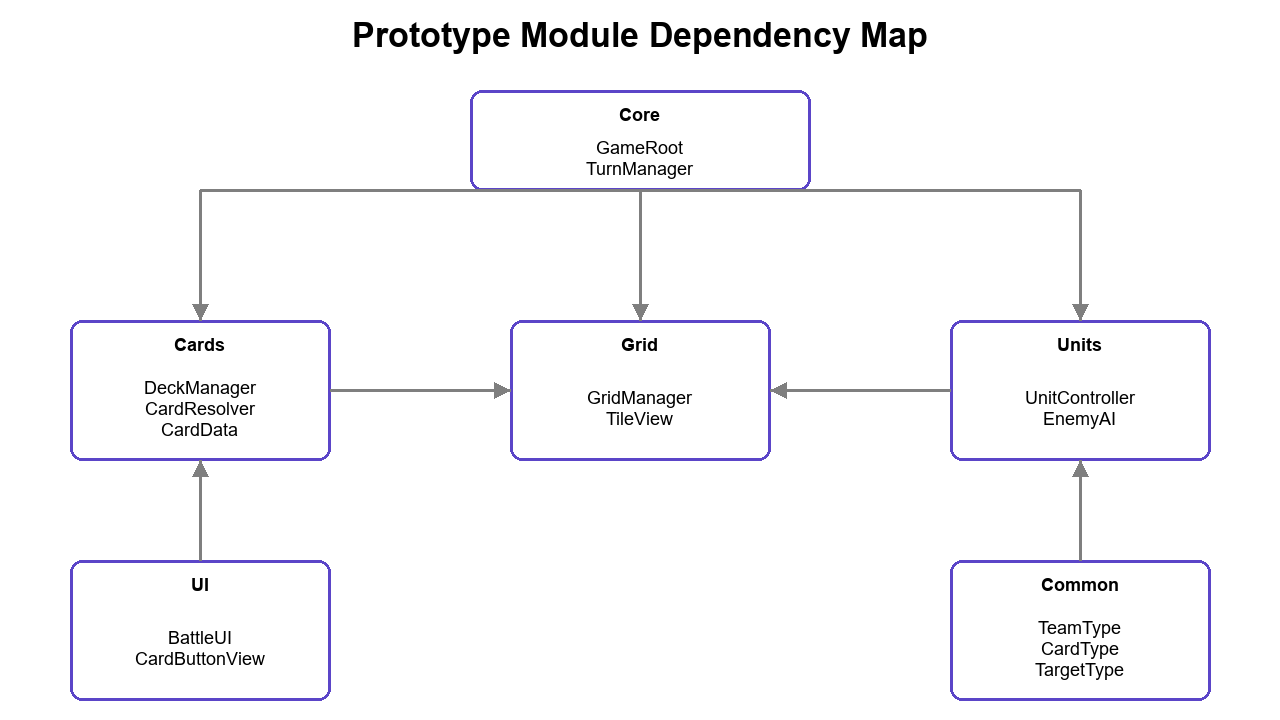
\includegraphics[width=0.93\textwidth]{media/module-map-wr1-style.png}
\caption{Simplified module dependency and responsibility map}
\label{fig:module-map}
\end{figure}

Figure~\ref{fig:module-map} is included to explain code responsibility split rather than runtime event order. It shows that dependencies flow inward toward a small number of managers instead of outward into a large inheritance tree. This is consistent with the project goal of a reportable, traceable prototype rather than a content-heavy tactics framework.

\subsection{Runtime Responsibilities Beyond the Diagram}

The responsibility map is intentionally simplified, so the feature-level role of each main script is summarised below:

\begin{itemize}
\item \textbf{\texttt{GameRoot}.} Registers the pre-placed units in the scene, links the managers together, and provides the starting point for the playable battle slice.
\item \textbf{\texttt{TurnManager}.} Controls player and enemy phase transitions, remaining card plays, start-of-turn draw behaviour, and the battle-end gate introduced by the prototype-accuracy fix.
\item \textbf{\texttt{GridManager}.} Builds the 6x6 board, tracks tile occupancy, and answers movement or target-range queries used by cards and AI.
\item \textbf{\texttt{DeckManager}.} Owns the starter deck, draw pile, discard pile, and current hand shown in the battle UI.
\item \textbf{\texttt{CardResolver}.} Converts \texttt{Move}, \texttt{Strike}, \texttt{Guard}, and \texttt{Push} into explicit runtime effects so card behaviour stays easy to trace and test.
\item \textbf{\texttt{UnitController}.} Stores team, hit points, guarding state, and grid position, and exposes the small set of combat operations needed by the current prototype.
\item \textbf{\texttt{EnemyAI}.} Produces the deterministic enemy response used in WR2, keeping target choice and movement logic simple enough to observe clearly during demonstration.
\item \textbf{\texttt{BattleUI} and \texttt{CardButtonView}.} Handle card selection, click routing, prompts, and log updates so the player can see the state changes caused by the core systems above.
\end{itemize}

\section{Critical Implementation Choices}

The most important implementation choices in the current prototype are:

\begin{itemize}
\item \textbf{Single self-contained battle.} Options considered: one battle scene versus multi-scene campaign flow. Chosen option: one battle scene, because it provides a complete vertical slice for WR2 without spending time on navigation and persistence. Trade-off: broader progression is postponed.
\item \textbf{Shared unit runtime model.} Options considered: one shared controller versus separate player/enemy hierarchies. Chosen option: one shared \texttt{UnitController} so that health, guarding, movement, and grid state remain easy to trace. Trade-off: the model is less specialised than a longer-term production structure.
\item \textbf{Explicit card resolver.} Options considered: \texttt{enum}-driven explicit logic versus a generic card-effect hierarchy. Chosen option: one resolver that interprets \texttt{CardType}, because the starter set is small and benefits from readable switch-based logic. Trade-off: a larger future card set would eventually need refactoring.
\item \textbf{Deterministic enemy AI.} Options considered: nearest-target movement versus broader tactical AI. Chosen option: deterministic nearest-target behaviour, because it is predictable, testable, and easy to explain in WR2. Trade-off: the enemy behaviour remains strategically shallow.
\item \textbf{Prototype-first UI and input path.} Options considered: a full Unity UI pipeline versus the current hybrid prototype UI with Input System and board raycasts. Chosen option: the hybrid path, because it was faster to wire into the existing scene and sufficient for WR2 reporting. Trade-off: UI consistency and polish remain limited.
\item \textbf{GitHub-first collaboration after repository cleanup.} Options considered: continue closing WR2 on a mixed local clone versus migrate report-closeout work onto a cleaned GitHub workflow with explicit PR rules. Chosen option: move current collaboration onto the cleaned GitHub repository, record the review policy, and keep earlier local/Overleaf/WeChat-era activity in supporting notes. Trade-off: current closeout work is now traceable through merged pull requests, but some earlier process evidence still relies on reconstructed notes and the task-board trail remains weaker than the repository history.
\end{itemize}

The most important strategic choice was to treat the prototype as implementation evidence rather than as the start of a fully general tactics engine. That choice explains why the runtime modules are explicit, why the card system is intentionally narrow, and why some features were marked as deferred instead of hidden behind partial abstractions. For WR2, this is a strength: the implementation remains aligned with the report, the frozen snapshot, and the current demonstration scope.
